% SPDX-License-Identifier: Apache-2.0
\documentclass[11pt,letterpaper]{article}
\usepackage[margin=0.85in,headheight=15pt]{geometry}
\usepackage[T1]{fontenc}
\usepackage[utf8]{inputenc}
\usepackage[english]{babel}
\usepackage{lmodern,microtype,amsmath,amssymb,booktabs,longtable,tabularx,array}
\usepackage{graphicx,xcolor,fancyhdr,enumitem,hyperref,url}
\definecolor{ink}{HTML}{17213B}
\definecolor{accent}{HTML}{5042A0}
\definecolor{muted}{HTML}{586277}
\definecolor{pale}{HTML}{F3F1F9}
\hypersetup{colorlinks=true,linkcolor=accent,urlcolor=accent,citecolor=accent,
pdftitle={AGI ALPHA Flywheel: Useful Delivery Before Capability Investment},
pdfauthor={AGI ALPHA research; AI-assisted research and engineering}}
\setlength{\parindent}{0pt}
\setlength{\parskip}{6pt}
\setlength{\emergencystretch}{3em}
\setlist{nosep,leftmargin=*}
\renewcommand{\arraystretch}{1.18}
\pagestyle{fancy}\fancyhf{}
\fancyhead[L]{\small\textcolor{muted}{AGI ALPHA / DISCOVER THE WORK}}
\fancyhead[R]{\small\textcolor{muted}{Research edition / 26 October 2026}}
\fancyfoot[L]{\footnotesize\textcolor{muted}{Executed public work; simulated markets; no paid customer trial}}
\fancyfoot[R]{\thepage}
\newcommand{\code}[1]{\texttt{\small #1}}
\newcommand{\ev}[1]{\texttt{\small\detokenize{#1}}}
\newcolumntype{Y}{>{\raggedright\arraybackslash}X}
\begin{document}
\selectlanguage{english}
\thispagestyle{empty}
{\small\bfseries\color{accent} AGI ALPHA FLYWHEEL \quad / \quad SUCCESSOR $\Omega$ HARNESS}
\vspace{0.8cm}

{\Huge\bfseries\color{ink} Useful Delivery Before\\[5pt] Capability Investment}

{\Large Discover the work. Build the advantage.}

{\large A bounded portfolio study of API response assurance and transit-feed qualification}

\vspace{0.4cm}
\textbf{Research date:} 26 October 2026. \quad
\textbf{System base:} AGI-Alpha-Agent-v0, commit \code{882456a}.

\textbf{Status:} Reproducible public-data research with useful scoped outputs. No customer purchase,
live ENS validation, contract settlement, or realized commercial return is asserted.

\begin{abstract}
We searched six materially different job families and executed two scoped offerings before
writing the paper. A REM transit-feed packet passes canonical structural validation and 86
independent reconciliation checks, while retaining 1,565 warnings. Three new API release
questions are accepted in all four compared approaches; three additional planned questions
remain source-acquisition failures. The retained conventional workflow is faster than the
Workbench full index, incremental registry and graph composition. Two competent recipients
reconstruct equivalent methods before receiving the asset. The original transfer control is
content-identical; a separately frozen changed-content follow-up is accepted by the narrow
system workflow but stopped by the second recipient's stricter input validator.

A source-frozen finite-cash simulation uses these measurements and explicitly assumed demand,
attention, competition and cost conditions. Across 384 paired worlds and 1,536 policy histories,
none produces positive ordinary operating surplus or funds a capability investment. The most
favorable cell averages a \$391.55 operating loss and a \$515.97 loss after its modeled opening
costs. Actual collections are zero and complete actual costs remain unknown. The supported
result is useful scoped delivery with preserved reusable engineering and a negative test of
the declared commercial cycle, not automation savings established against timed humans,
scarce transferable capability, graph advantage, modeled self-financing succession or realized
commercial success.
\end{abstract}


\vspace{0.3cm}
\colorbox{pale}{\parbox{\dimexpr\linewidth-2\fboxsep\relax}{
\textbf{Decision supported by the engineering evidence.}
Retain the useful delivery artifacts and the simpler conventional workflow. Do not finance the
tested Workbench index or graph composition on an unmeasured scarcity premium. A future investment
must first establish a buyer-relevant gap that competent existing tools do not already close.
}}

\vfill
\textbf{Authorship and review.} AI-assisted research and engineering coordinated through
\href{https://github.com/MontrealAI/AGI-Alpha-Agent-v0/issues/4850}{AGI ALPHA issue \#4850}.
Separate same-session agents constructed comparators, reviewed engineering, and audited economics.
This is not independent external peer review. No transit publisher, Docker maintainer, or buyer
has endorsed the service.

\textbf{Evidence companion.} Frozen source, original public inputs and licenses, accepted outputs,
failed trials, process receipts, transfer records, the finite-cash simulator and its ledgers,
and an offline English/French demonstration accompany this paper.
\newpage
\tableofcontents
\newpage

\section{The customer work and the result}

The commercial hypothesis was a connected sequence: useful work, accepted efficient delivery,
collected surplus, an affordable capability investment, and better fresh work. The study did not
treat an implementation, a signed fixture, a benchmark count, or avoided labor as revenue. It
first screened six different job families and executed two finalists using the existing
SUCCESSOR Workbench where its actual extension interface permitted it.

The first offering delivers an exhaustive, source-bound inventory of declared GET 2xx JSON
schema facts within a supported grammar, between two API specifications. It supports a precise review task:
identify the response fields and constraints that changed, trace each change back to its source,
and decide which client checks require attention. It does \emph{not} establish live-client
compatibility. The second offering delivers a REM GTFS ingestion packet for a specified week:
canonical-validator results, route/date trip counts, independent reconciliation, preserved
warnings and an explicit structural disposition.

These outputs have identifiable beneficiaries: integration maintainers and transit-data
ingestion teams. They use real public source artifacts and support concrete review or ingestion
actions. They were not commissioned by those beneficiaries. Their usefulness is supported by
the completed artifacts and technical acceptance, while their willingness to pay remains
unobserved. The API dossier is narrower than the initially envisioned consumer migration packet;
the later source-bound consumer appendix makes the remaining gap explicit.

\begin{table}[htbp]\small
\caption{All six locked API questions, including blocked deliveries. Counts are structural facts, not customer incidents.}
\begin{tabularx}{\linewidth}{@{}p{0.28\linewidth}p{0.18\linewidth}p{0.12\linewidth}Y@{}}
\toprule Question & Old / new nodes & Changes & Four-arm disposition\\ \midrule
v20.10.0 $\rightarrow$ v23.0.0 & 2,233 / 2,341 & 489 & 4 / 4 scoped pass \\
v23.0.0 $\rightarrow$ v24.0.0 & 2,341 / 2,343 & 8 & 4 / 4 scoped pass \\
v24.0.0 $\rightarrow$ v25.0.0 & 2,343 / 2,408 & 70 & 4 / 4 scoped pass \\
v26.0.0 $\rightarrow$ v27.0.0 & -- & -- & Source path 404; 0 / 4 delivered \\
v27.0.0 $\rightarrow$ v28.0.0 & -- & -- & Source path 404; 0 / 4 delivered \\
v28.0.0 $\rightarrow$ v29.0.0 & -- & -- & Source path 404; 0 / 4 delivered \\
\bottomrule\end{tabularx}
\end{table}

The primary delivered three distinct dossiers, accepted in all four arms: 12 accepted arm/question
outputs out of 24 planned. Three other questions were blocked by two locked source-path 404s.
On available inputs, conditional technical acceptance was 12/12. The intent-to-deliver fraction
was 12/24. These denominators answer different questions and are both retained.

The REM packet covers 26 October--1 November 2026, in GTFS local service dates. Its original
feed version is 20260520, with declared coverage through 31 December 2026. It contains three
routes, 1,081 trip templates and 19,069 stop-time rows. The supported calendar expansion yields
443 scheduled trip instances on each weekday, 323 on Saturday and 315 on Sunday: 2,853 in
total. There are 21 route/date cells and seven daily groups in one delivery.

The canonical MobilityData validator 8.0.1 reports zero errors, 1,565 warnings and one informational
notice. Eighty-six independent SQLite reconciliation checks pass. The disposition is
\textbf{SCOPED STRUCTURAL PASS}, with warnings retained for interpretation. This permits
structural ingestion of the supplied snapshot within the declared scope; it does not certify
real-time service or independently verify the timetable against actual operations.
The external Java/Python stages and actual Workbench aggregation have 21.558 measured command
wall seconds and 23.718 CPU seconds in total, excluding unmetered authoring and attention.
The Workbench aggregation command contributes 0.115 wall seconds and 0.123 CPU seconds.


\subsection{A consequential scope boundary}

The consumer review considered legacy Docker Compose 1.29.2 and Docker Engine 26. Official
Docker documentation describes the omission of \code{Container} and \code{ContainerConfig}
from image inspection at API version 1.45 and later \cite{docker-deprecation}. The archived
v25 and v26 specifications used during construction still contain these fields. A structural
specification diff therefore cannot certify this behavior change or claim to have detected it.
The accompanying consumer appendix binds the authentic consumer location, the archived schema
evidence and the official documentation. In the previous-container path of Compose 1.29.2,
line 1579 directly indexes \code{ContainerConfig} \cite{compose-source}. The unmodified,
AST-extracted function returns an empty binding result for the present-key fixture and raises
\code{KeyError} for the omitted-key fixture even when \code{Config} is present. Its conditional
decision is to require a maintained consumer and staging evidence when this path uses API 1.45
or later. Static and extracted-function evidence are labeled as such; no live Docker service
or full application migration was executed for this claim.

This boundary is economically relevant. A low-cost schema report is not equivalent to a
finished migration assurance service. The modeled offering, human comparator and competitors
all use the same limited dossier scope. Broader assurance would require additional implementation,
verification and residual attention, whose costs cannot be erased by changing the product label.

\section{Discovery before commitment}

\subsection{Budget, selection and demand evidence}

The declared budget was six job families, no more than two development prototypes, two
capability candidates, a 35-minute discovery window, a 45-minute window for each prototype,
and 60 seconds per production process. These are bounded research allowances, not dollar
budgets or metered human work. Agent intervals overlap and are never summed into a labor invoice.
Finalists were selected from primary-source evidence and feasibility before confirmatory
outcomes. Selection and later source freezes are retained separately.

API releases are authentic recurring triggers: GitHub explicitly directs maintainers to review
breaking changes, update integrations and test them \cite{github-versions}. Transit publication
is also recurrent: TransLink describes weekly feed updates and at least four seasonal changes
per year, while Caltrans describes interpreting feed-quality evidence with providers
\cite{translink,caltrans}. These facts establish recurring work classes, not sales counts for
this enterprise. The selected execution feed was REM under its embedded CC BY 4.0 license,
not TransLink data with additional commercial-use conditions.

\begin{table}[htbp]\small
\caption{Portfolio ranked before finalist outcomes. Ordinal judgments are researcher estimates.}
\begin{tabularx}{\linewidth}{@{}p{0.05\linewidth}p{0.23\linewidth}YY@{}}
\toprule
Rank & Family / beneficiary & Complete action and existing alternative & Selection judgment\\
\midrule
1 & API assurance / integration owners &
Source-bound upgrade review; oasdiff and competent developers already exist. &
Selected: public versioned inputs and exact acceptance are feasible; consumer completeness and differentiation are uncertain.\\
2 & GTFS assurance / feed ingestion teams &
Scoped ingestion disposition and service-date reconciliation; canonical MobilityData validator. &
Selected: recurring schedules, reusable integration, permissive input available; no paid demand observed.\\
3 & SQL performance repair / analytics maintainers &
Equivalent query or resource fix; DuckDB optimizer and expert tuning. &
Authentic issue \#22474, but its large reproducer exceeds the local screen budget.\\
4 & Accessibility repair / website maintainers &
Scoped repair plus task assessment; automated tools and knowledgeable evaluators. &
Whole-site acceptance cannot honestly be reduced to an automated score.\\
5 & Numerical qualification / scientific users &
Accuracy dossier tied to a real downstream decision; mature solvers and NIST reference data. &
Reference cases alone are a benchmark, and the active numerical lane was excluded.\\
6 & Generic source migration / library maintainers &
Patch with regression tests; Ruff NPY201 and existing codemods. &
Strong public alternatives and overlap with dependency work reduce expected additional value.\\
\bottomrule
\end{tabularx}
\end{table}

The excluded families were not demonstrated to be commercially absent. SQL repair lacked
a justified local-scale reproducer within the budget; accessibility had a difficult
assessment boundary; numerical reference testing lacked a specific buyer job; generic migration
had strong existing tooling. W3C's requirement for knowledgeable human evaluation and NIST's
reference-data purpose informed those choices \cite{w3c,nist}. The complete matrix preserves
buyers, triggers, human workflows, alternatives, demand evidence, automation bottlenecks and
uncertainty for every candidate.

\subsection{Why the second finalist was not expanded}

The REM packet is a complete exploratory delivery, but this run did not establish a scarce
GTFS skill, a second fresh feed comparison, a measured human-only advantage, or an economical
transfer. Conventional validation was already strong. Expanding this candidate into a second
unvalidated market model would have overstated the evidence. It remains a useful retained
composition and a future candidate if actual recurring ingestion requirements justify it.
The API family supplied the bounded repeated comparison, not a presumed commercial winner.

\section{What was constructed and what was already available}

The starting system had public-data Workbench adapters, canonical mission and Jobs draft
compilation, evidence hashing, prior graph/authority fixtures, and general-purpose programming
tools. It did not contain this source-bound API dossier adapter. That absence did not imply that
other agents lacked the capability: two separate agents received reasonable search, conventional
tools and reconstruction budgets, and both built equivalent analyzers.

The first retained asset is a deterministic JavaScript response index and dossier adapter.
It enumerates successful GET JSON response schemas, local references, properties, arrays,
additional-property schemas and structural composition branches. Facts, source pointers and
reference chains remain separate. Unsupported constructs are disclosed. The second asset
adds dependency-aware reuse of source-bound response subtrees. It invalidates affected roots
when transitive source dependencies change. It retains a private current-session authenticity
check for issued indexes; imported or tampered caches do not silently acquire trust.

Important corrections were required during construction: complete transitive source binding,
explicit unsupported-keyword reporting, ownership of asynchronous inputs, private cache-chain
trust, refusal to overwrite output directories, and safe UTF-16 fragment boundaries. Original
source snapshots and failed controls remain in the companion. These are validated engineering
improvements. They are not claims of a newly discovered indexing algorithm.

The exact contract required executable construction and checking of version binding,
fragment reconstruction, evidence linkage and independent replay. The quick independent
reconstructions do not establish a scarce capability or superiority over ordinary agent/tool
workflows. Established
public tools, however, already perform substantial API analysis. The study therefore compares
against a retained conventional builder and a pinned oasdiff supplement, not against an
unprepared agent with an empty skill directory.

\subsection{Existing system integration}

API computation runs as an actual pure-JavaScript extension of the existing Workbench.
The adapter returns source-bound artifacts, and the existing engine compiles seven unfunded
Jobs drafts, checks the pack, and preserves public-local execution scope. The GTFS stage is
different: an external Java validator and Python/SQLite analysis precede an actual Workbench
aggregation of the 21 route/date rows into seven daily totals. No arbitrary native Python
dispatcher is implied.

These concrete integration points are the operational use of the existing TRANSFORMATIONAL
INTELLIGENCE $\infty$ and SUCCESSOR $\Omega$ foundations in this study.
The four reviewed repositories retain their roles. AGI-Fleet-Linux remains a deployment and
fleet foundation; AGIJobsv0 and AGIJobManager retain their existing Jobs contracts, governance
and settlement boundaries. This study does not establish installed four-product qualification.
It does not convert the system's unfunded drafts into operational jobs, approve execution,
or move funds.

\section{Comparisons that answer different questions}

\begin{table}[htbp]\small
\caption{Four distinct estimands. An answer to one does not imply the others.}
\begin{tabularx}{\linewidth}{@{}p{0.2\linewidth}YY@{}}
\toprule
Comparison & What is compared & Evidence available here\\
\midrule
Customer value & Equivalent competent human-only work, using conventional software, versus automated delivery &
Executed machine resource costs; human duration and residual attention are explicit scenarios, not a timed trial.\\
Competitive value & Offering versus strongest practical software or AI-assisted alternative &
Independent retained Python workflow; pinned converted-oasdiff supplement; buyer options in the simulation.\\
Investment value & Same enterprise before and after acquiring the capability &
Measured A/B/C/D cost deltas, complete hypothetical acquisition costs, finite-life gate. No recurring reconstruction charge.\\
Network value & Independent agents versus shared registry versus graph-guided reuse &
Registry and graph receive identical skills, evidence and dependencies; capability recipients retain their original programs.\\
\bottomrule
\end{tabularx}
\end{table}

\subsection{Freeze, confirmation and acceptance}

The production manifest froze 61 files at 21:09:19 UTC, before fresh inputs were acquired.
It binds source, acceptance, protocols, fixtures, dependencies and construction evidence.
The six primary version pairs and two transfer pairs were fixed separately. Each primary
arm ran once in rotating order, with a 60-second process bound. Acquisition failures,
timeouts and rejected outputs were not replaced or repaired into the primary result.
The driver checks source and input identities immediately before production and verification,
then checks custody again at the end.

Acceptance independently re-enumerates the supported schema facts and checks every changed
tuple, old/new node counts, source locations, reference provenance, input digests and output
reconstruction. Missing, extra or duplicate differences fail. Workbench packs are inspected
through their real interface. The original conventional workflow has its own separately
authored breadth-first verifier. Same-session independence limits shared implementation
mistakes; it is not external certification.

The primary sequence is historical public work, fresh to construction. It is not six current
customers, six independent organizations or a population estimate. Release lineage is correlated.
Only one timing is retained per arm and case; minor timing differences cannot establish a
general performance ordering.

\begin{table}[htbp]\small
\caption{Primary executed service resources. Includes production, independent verification and packaging; shared retrieval is reported separately.}
\begin{tabularx}{\linewidth}{@{}Yrrr@{}}
\toprule Arm & Accepted / planned & Total CPU s & CPU s / accepted\\ \midrule
A: Retained conventional & 3 / 6 & 1.274743 & 0.424914 \\
B: Workbench full & 3 / 6 & 4.658206 & 1.552735 \\
C: Incremental registry & 3 / 6 & 5.304753 & 1.768251 \\
D: Incremental graph & 3 / 6 & 4.863663 & 1.621221 \\
\bottomrule\end{tabularx}
\end{table}

The complete primary campaign used 16.139765 CPU seconds and
15.012749 elapsed seconds. Its driver overhead was
0.038400 CPU seconds, allocated separately from the table.
The all-input acquisition session used 4.806423 CPU seconds and 7.387453 elapsed seconds.
Source availability, normalized bytes, licenses and failed URLs are preserved in the input manifest.


\begin{figure}[htbp]\centering
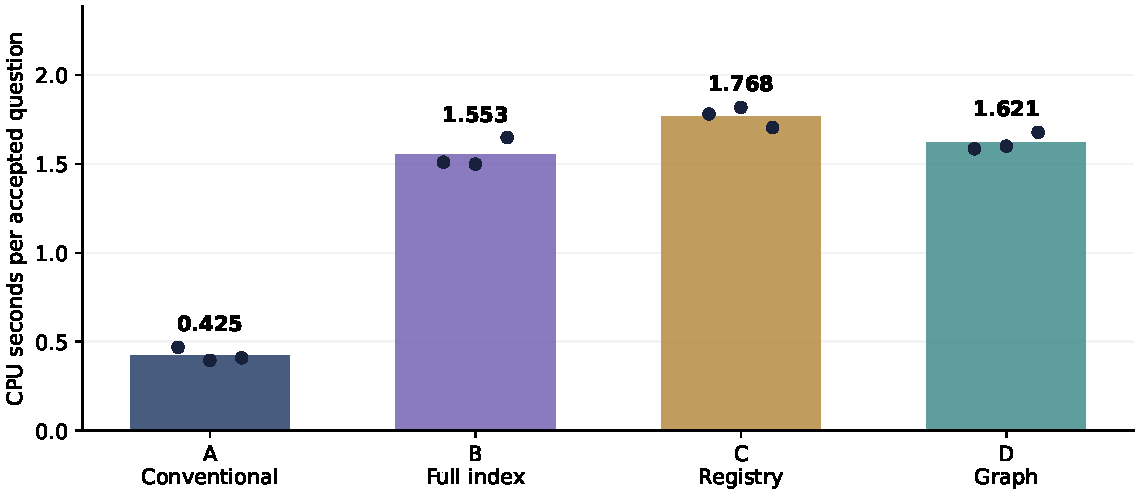
\includegraphics[width=0.9\linewidth]{figures/primary-cpu.pdf}
\caption{Each dot is one accepted primary question; bars are their mean. Complete compared delivery
includes independent verification and packaging. Three blocked questions per arm remain in the
intent-to-deliver denominator but do not become zero-duration successful jobs. One pass per case
does not establish a latency distribution. Shared acquisition and research costs are separate.}
\end{figure}

All four arms agree on the exact changed fact tuples and source provenance. The conventional
builder is faster in every available primary question. Incremental reuse does not improve the
primary average over the full Workbench index. The graph mean is slightly below the registry mean
in this single run, but it creates no additional accepted work and supplies no independently
identified planning advantage. Both remain slower than the conventional builder.

The public-tool supplement strengthens the alternative. After validated Swagger2-to-OpenAPI
conversion, oasdiff 1.34.1 reports 102, 5 and 0 breaking findings and 365, 9 and 77 changelog
items on the three available pairs. Its broader request/response/media coverage is not the same
acceptance task as the structural dossier. Raw Swagger2 supplied to the OpenAPI3 validation contract produced 15, 1 and 0
findings despite 103--105 validation errors; default exit zero therefore did not establish a
valid result. A YAML parser failure on v20 was preserved, then a separately labeled follow-up
used the existing frozen normalized JSON. All 27 supplemental commands, including invalid and
failed attempts, used 6.280 seconds wall and 8.923 CPU seconds. No primary producer was rerun.


\subsection{Transfer to competent recipients}

Recipient one built the conventional Python workflow before viewing donor code, after public-tool
search. Its observed construction interval was 390.812 seconds. Recipient two independently
built another Python implementation in 348.622 seconds. These intervals include tools, reasoning,
tests, waits and some context switching; they are neither human task times nor inference invoices.
Recipient two integrated the donor module in 44.568 seconds, with 0.956 CPU seconds in the
recorded integration commands. This supports only a hypothetical possibility of avoiding
initial work for a future recipient. Both tested recipients had already paid the reconstruction
effort; no such saving was realized here. It does not justify charging reconstruction on every future job.

\begin{table}[htbp]\small
\caption{Original and separately declared exploratory transfer. No original failure is replaced.}
\begin{tabularx}{\linewidth}{@{}p{0.25\linewidth}YY@{}}
\toprule Question & Frozen system / recipient one & Independently built recipient two\\ \midrule
v23.0.0 $\rightarrow$ v23.0.6 &
Four arms pass, but normalized inputs are byte-identical. No changed-work evidence. &
Own, received full and incremental methods agree on 2,341 nodes and zero changes.
Execution CPU: 0.115, 0.245 and 0.262 seconds before shared validation.\\
v27.0.0 $\rightarrow$ v27.5.1 &
Locked source acquisition fails; all four arms remain unexecuted. &
All three methods remain unexecuted.\\
Exploratory v27.5.1 $\rightarrow$ v28.0.0 &
Four narrow-scope outputs pass with 332 changes. CPU: A 0.594, B 2.797,
C 2.201, D 1.920 seconds, including verification/packaging. &
Existing raw-Swagger validator rejects a required/properties relationship.
All three efficacy attempts remain NOT RUN; the validation failure costs 0.664 CPU seconds.\\
\bottomrule
\end{tabularx}
\end{table}

The exploratory follow-up was separately frozen and posted before its outputs, selected only
because both already acquired inputs were available and had different byte identities. It
used unchanged implementations and acceptance. Its 7.545 CPU seconds and 7.106 elapsed seconds
are new research execution; already paid acquisition is not charged again to the historical
book. Browser QA overlapped part of the parent run, limiting interpretation of its wall timing.
No performance rerun or input replacement was made, and no secondary result enters the primary
market calibration.

Recipient two's selected validator rejects a required \code{UnpackedSize} member that is not
declared under \code{properties}. Read-only standards adjudication found that this particular
check is stricter than the normative relationship: OpenAPI 2 adopts Draft 4's \code{required}
unchanged, which constrains instance membership rather than requiring a schema-property
declaration \cite{oas2,draft4}. That does not adjudicate whole-document validity. The original
validator HOLD remains authoritative for this recipient's frozen procedure. The difference
is an input-qualification boundary, not evidence that the donor completed a broader task or
that this recipient received a useful new capability.


The recipient designs differed: one used an independent retained constructor plus breadth-first
verification; the other built its own response inventory and then a thin donor wrapper.
Both already had effective capability before transfer. The surviving tag-held-out minor-version case
has byte-identical normalized specifications and is a content-identity control; the second declared
transfer case is acquisition-blocked. Those original tests do not establish transfer to
meaningfully changed work. A separately registered one-pair exploratory follow-up uses
different-content inputs without changing either implementation; its results are reported
separately and excluded from economic calibration. Neither recipient was actually incapable,
so this study does not establish valuable positive transfer to such a recipient or skill scarcity.

\section{Economic conditions, accounting and investment}

Actual collections are zero. Actual complete inference, construction, review, support and
maintenance bills are unavailable. The economic study therefore uses executed resource
measurements as inputs to an explicitly assumed buyer-and-competitor model. It does not infer
an invoice from agent wall time, a price from a desired savings ratio, or demand from the number
of generated rows.

The sourced wage anchor is the BLS May 2025 median annual wage of \$135,980 for software
developers \cite{bls}. Dividing by an assumed 2,080 annual hours gives \$65.375 per hour.
That is a US wage modeling convention, not a Quebec quotation, a fully loaded professional
rate or a measured productive hour. Exact-job human durations, customer willingness to pay,
integration and residual attention were not observed. Their assumed ranges are declared
before simulated outcomes.

\subsection{Separate cost books}

\begin{enumerate}
\item \textbf{Marginal execution:} production, independent verification, packaging, failed attempts,
source checking and acquisition resources. Internal receipts are not added to outer process-tree
CPU again.
\item \textbf{Recurring operation:} buyer and provider onboarding, residual attention, support,
business overhead, corrections, tool costs and maintenance. These are modeled when not executed.
\item \textbf{Full prospective delivery:} recurring costs plus allocated ordinary setup.
Experimental four-arm sharing is removed when costing a standalone enterprise.
\item \textbf{Incremental capability investment:} construction, failed construction, integration,
validation, inference allowance, maintenance and useful-life limits, charged once on acquisition.
\item \textbf{Historical research:} discovery and failed discovery, kept separate from prospective
deployment and historical recovery. Earlier studies' scenario costs are preserved as prior
evidence and are not silently charged again as current invoices.
\end{enumerate}

The root acquisition session fetched or reused each registered source once. Experimental
allocations share that work across version appearances and four arms; a standalone policy bears
its own service share rather than receiving a four-arm discount. The companion retains both
interpretations and the small driver overhead. Output rows, structural changes and seven Jobs
drafts are not additional customers.

\subsection{Frozen buyer-and-competitor experiment}

The source and calibrated inputs were frozen and posted before the first economic run.
There are 24 conditions, from three buyer arrival probabilities (0.025, 0.125 and 0.25 per
buyer-week), two buyer integration conditions (0 and 15 minutes), two competitor conditions
(equal and stronger), and two full-cost bundles (low and reference). Sixteen paired seeds
produce 384 worlds; each contains four separate counterfactual policy histories over 52 weeks. The
24-buyer pool is an assumed simulation population, not an estimated addressable market.

Each enterprise starts with \$1,000 seed capital and a \$200 investment reserve. The reserve
limits discretionary capability investment; it does not prevent ordinary obligations from
exhausting cash. Customer payments arrive two weeks after accepted delivery, with a modeled
0.98 collection probability. Unpaid expenses remain obligations. Receivables, seed and internal
transfers are not operating-generated investment funds. All book money uses integer cents;
investment benefit comparisons retain microdollar precision and conservative cash-rounding effects.

The common 0.5 source-availability condition reflects the six locked questions' 3/6 observed
availability, solely as a scenario calibration. A blocked source incurs acquisition and
five assumed triage minutes, no delivery retry, onboarding, support or invoice. Available
jobs use the observed 3/3 conditional acceptance plus a 0.98 execution-stress assumption
and at most two attempts. These are scenario mechanisms, not estimated population probabilities.
Human-only/public-DIY delivery uses the same assumed 5, 15 or 45 minutes with competent
conventional software. No extra undocumented speed multiplier makes that baseline artificially weak.

The enterprise and equal AI-assisted competitor use the same prospective cost function and
tariff rule. The tariff is the smallest member of a labor-equivalent grid that covers expected
collected-job cost at three intended orders per week. That cost includes source rejection,
execution, correction, support, allocated onboarding, weekly business/maintenance/tools, ordinary
setup and compute. A neutral paired draw resolves equal paid offers. The stronger competitor
has an explicit 0.6 labor-efficiency assumption. At week 20 competitors can copy, reduce effort
and cut prices subject to their prospective cost floor. Buyers can self-serve or decline;
orders, delivered jobs, customer avoided labor and collected revenue remain separate.

The low bundle assumes two residual provider minutes per attempt, 0.5 support minutes per order,
five provider-onboarding minutes, five weekly business minutes, two weekly maintenance minutes
and \$1 weekly tools. The reference bundle uses five, two, fifteen, fifteen and five minutes,
respectively, and \$5 weekly tools. Their modeled historical discovery/setup openings cost
\$124.42 and \$502.63. These labor and inference allocations are not observed invoices.
Candidate construction performed in the research remains an unknown actual historical cost;
the counterfactual enterprise pays the candidate's modeled incremental cost once only if
it purchases that asset. Adding omitted nonnegative historical research costs cannot improve
the negative recovery results.

All policies begin with retained conventional A. Policy A makes no purchase; B permits A to B;
C permits A to B to C; D permits A to B to D, with graph costs itemized in its second asset.
The second purchase cannot bypass its first prerequisite. Investments have a 26-week useful
life, an eight-week lookback and earliest investment week eight. Forecasts discount observed
reuse and are bounded by remaining useful life. These operating policies are distinct from
the separately reported prebuilt A/B/C/D engineering comparison.

Before outcomes, synthetic and independent review corrected asymmetric tariff treatment,
unmatched DIY time, acquisition sharing, source-blocked costs and cash rounding. The initial
drafts and failed signed-zero control are retained. No simulated profit was used to tune these
changes. All 26 final synthetic controls passed; there was one primary market run and no
favorable substitute campaign.

\subsection{The ordinary service fails before the investment loop}

\textbf{No world produces positive ordinary operating surplus.} Across all 384 worlds,
available earned investment funds remain exactly zero in every week. No first or second
capability is acquired, and no succession repays. The four policy results are identical
because every policy retains A. This is an operating-demand/cost failure before a capability
funding event, not a claim that graph execution caused the losses.

\begin{longtable}{@{}llllrrr@{}}
\caption{All 24 primary economic conditions, 16 seeds each. Mean accepted jobs and USD results.
Policies A/B/C/D coincide because no purchase is admitted. I is buyer integration minutes.}\\
\toprule Demand & I & Competitor & Cost & Jobs & Operating & Project\\ \midrule\endfirsthead
\toprule Demand & I & Competitor & Cost & Jobs & Operating & Project\\ \midrule\endhead
low & 0 & strong & low & 0.00 & -448.76 & -573.18 \\
low & 0 & strong & reference & 0.00 & -509.20 & -1011.83 \\
low & 0 & equal & low & 1.00 & -447.18 & -571.60 \\
low & 0 & equal & reference & 0.00 & -509.20 & -1011.83 \\
low & 15 & strong & low & 0.00 & -448.76 & -573.18 \\
low & 15 & strong & reference & 0.00 & -509.20 & -1011.83 \\
low & 15 & equal & low & 0.81 & -445.54 & -569.96 \\
low & 15 & equal & reference & 0.00 & -509.20 & -1011.83 \\
reference & 0 & strong & low & 0.00 & -448.76 & -573.18 \\
reference & 0 & strong & reference & 0.00 & -509.20 & -1011.83 \\
reference & 0 & equal & low & 4.25 & -439.42 & -563.84 \\
reference & 0 & equal & reference & 0.00 & -509.20 & -1011.83 \\
reference & 15 & strong & low & 0.00 & -448.76 & -573.18 \\
reference & 15 & strong & reference & 0.00 & -509.20 & -1011.83 \\
reference & 15 & equal & low & 4.19 & -430.30 & -554.72 \\
reference & 15 & equal & reference & 0.00 & -509.20 & -1011.83 \\
high & 0 & strong & low & 0.00 & -448.76 & -573.18 \\
high & 0 & strong & reference & 0.00 & -509.20 & -1011.83 \\
high & 0 & equal & low & 8.75 & -410.80 & -535.22 \\
high & 0 & equal & reference & 0.00 & -509.20 & -1011.83 \\
high & 15 & strong & low & 0.00 & -448.76 & -573.18 \\
high & 15 & strong & reference & 0.00 & -509.20 & -1011.83 \\
high & 15 & equal & low & 9.75 & -391.55 & -515.97 \\
high & 15 & equal & reference & 0.00 & -509.20 & -1011.83 \\
\bottomrule\end{longtable}

The most favorable cell mean is high arrival, 15-minute buyer integration, equal competition
and low operating cost: 9.75 accepted jobs, \$153.28 simulated collections, \$391.55 operating
loss and \$515.97 modeled project loss. This is a post-run descriptive maximum, not a newly
selected confirmatory condition. Even the best individual world loses \$233.97 operating
and \$358.39 after opening costs: \$408.75 collected versus \$642.72 accrued operating costs
and \$124.42 opening costs. Its cash is \$655.70, unpaid obligations \$14.09 and receivables
\$32.70. Positive cash includes remaining seed and is not profit.

All reference-cost conditions exhaust cash and become insolvent at week 20. Their 19 charged
weeks accrue \$509.20 operating cost, in addition to \$502.63 opening cost, leaving \$11.83
unpaid. All low-cost/strong-competitor conditions collect nothing and lose \$448.76 in recurring
operation, or \$573.18 including opening costs. The model makes refusal, competition and
finite capital consequential rather than replacing missing sales with assumed transfers.

\begin{figure}[htbp]\centering
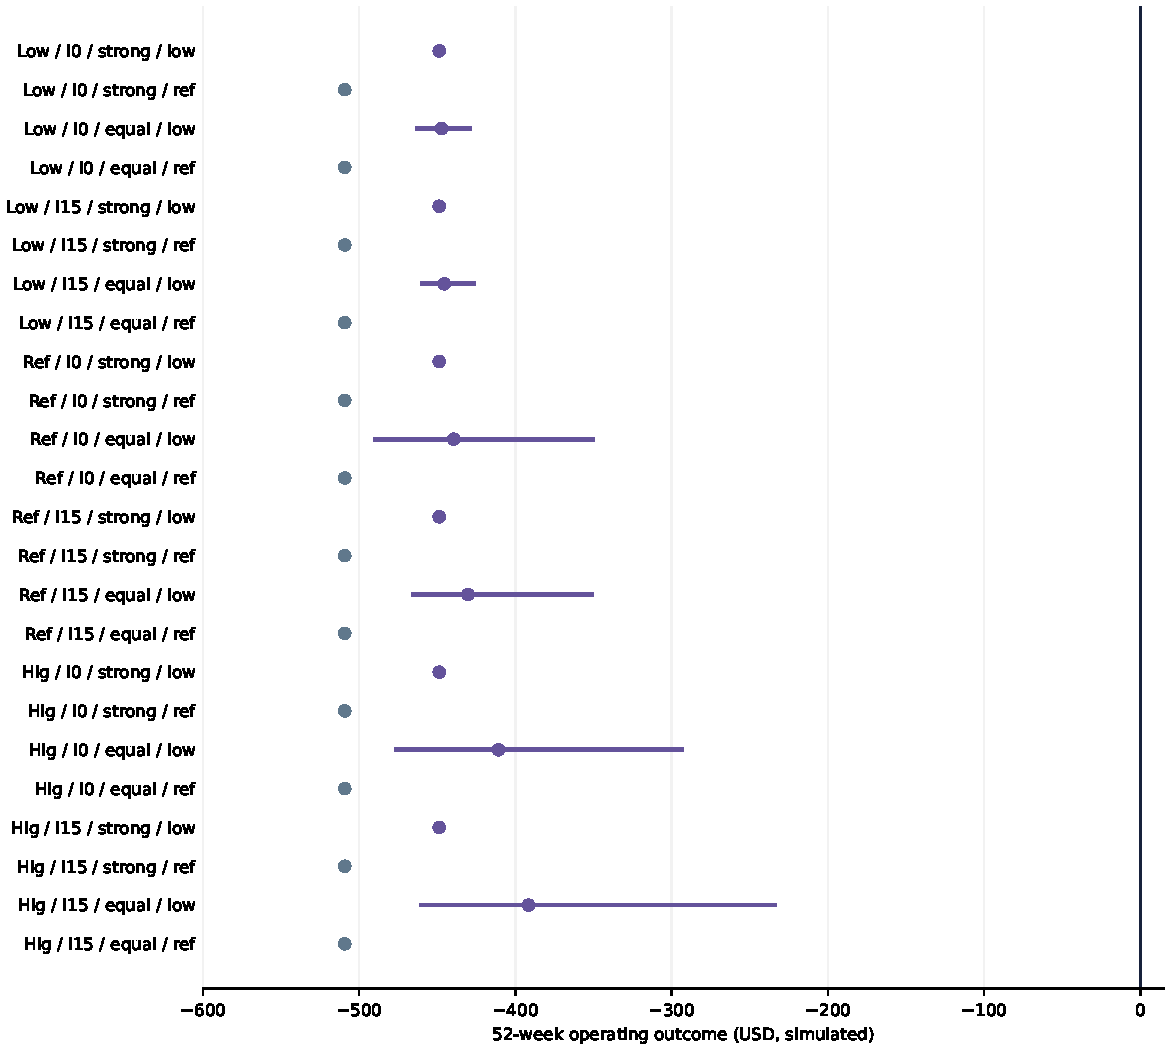
\includegraphics[width=0.95\linewidth]{figures/economic-cells.pdf}
\caption{All predeclared cells. Dots show mean operating outcome across 16 paired seeds; lines
show the full minimum--maximum range, not confidence intervals. Labels show demand, integration,
competition and cost bundle. Every range remains below zero. Reference-cost runs stop after
insolvency; they do not receive an extra seed injection.}
\end{figure}

\subsection{Cheap computation is not a complete service margin}

Including acquisition, failed source handling at the machine level and driver allocation, the
standalone mechanical CPU per accepted question is 1.547, 2.675, 2.891 and 2.744 seconds for
A/B/C/D. At the \emph{assumed} \$1 per CPU-hour, these are far below a cent. The actual billed
machine and inference costs are not known. Residual attention, low conversion and recurring
operation dominate the declared scenarios.

\begin{table}[htbp]\small
\caption{Prospective costing is not realized utilization. All dollar values below are modeled.}
\begin{tabularx}{\linewidth}{@{}Yrr@{}}
\toprule Quantity & Low bundle & Reference bundle\\ \midrule
Expected full prospective cost per collected job at reference utilization & \$15.48 & \$35.10\\
Resulting fixed grid tariff & \$16.35 & \$65.38\\
Historical discovery/setup opening & \$124.42 & \$502.63\\
First capability A to B, complete fixed incremental cost & \$135.77 & \$449.95\\
Second capability B to C, complete fixed incremental cost & \$119.43 & \$363.24\\
Second capability B to D, including graph increment & \$165.53 & \$509.46\\
\bottomrule\end{tabularx}
\end{table}

The best cell's actual modeled utilization produces approximately \$55.88 accrued recurring
cost per accepted job and \$68.64 including its opening allocations (ratios of cell totals).
Those figures differ from the \$15.48 prospective cost because competition and refusal prevent
the assumed reference utilization from being achieved. The grid's reference tariff jumps from
\$35.10 calculated cost to \$65.38, above the maximum modeled willingness to pay. This coarse
pricing choice contributes to refusal; it is a limitation of the tested policy, not empirical
evidence that a continuously priced offering cannot sell. No alternative price campaign was
introduced after observing these outcomes.

Human-only duration remains unmeasured. For example, the assumed 45-minute competent workflow
costs \$49.04 at the wage anchor; a \$16.35 service plus two buyer-review minutes costs \$18.53
before buyer integration. That conditional \$30.51 avoided cost is not observed savings,
enterprise revenue beyond the tariff, or available surplus. Shorter assumed human workflows
can rationally favor self-service. The diagnostic table varies residual attention over 2, 5 and
10 minutes and retains the unknown actual full-cost category.

\subsection{The proposed upgrades also lack a repayment case}

A to B adds 1.128 measured CPU seconds per available accepted question; B to C adds 0.216;
B to D adds 0.068. These signed deltas supply no positive CPU-only saving even at zero incremental
maintenance. The complete candidate investments therefore have no finite CPU-only break-even
reuse or repayment time. Adding the declared maintenance cannot improve that conclusion.
None was financed.

The separate C-to-D graph diagnostic has a 0.147-second observed CPU difference in the favorable
direction, without an added accepted job or identified planning gain. Even if that single-run
difference were stable and credited at \$1 per CPU-hour, the low \$46.10 graph increment would
require over 1.15 million reuses at zero maintenance with the frozen conservative microdollar credit (about 1.159 million under the conservative
cash-rounding diagnostic). Nonzero declared maintenance removes the finite repayment.
This is a sensitivity calculation, not evidence that the measured timing difference generalizes.

At an illustrative 156 execution reuses in 26 weeks, the low-cost A-to-B investment would need
about 0.90 minutes of additional paid attention avoided per reuse to cover its complete cost
and maintenance. No such saving was observed. This is a concrete measurement target for a
future capability test, not a benefit inserted into the present simulation.


\subsection{What an investment must repay}

Let $I$ be the complete incremental acquisition and validation cost, $\Delta c$ the signed
per-reuse execution saving, $m$ maintenance cost allocated per execution reuse, and $N_L$ feasible execution reuses
during useful lifetime $L$. A necessary condition for repayment is
\[
          N_L(\Delta c-m)\ \geq\ I,\qquad \Delta c-m>0.
\]
Cash availability is a separate condition. Collected operating funds must cover $I$ after
unpaid obligations and the reserve; seed principal and uncollected receivables are not available
earned funds. If net saving is nonpositive, no finite break-even reuse or repayment time exists.
If a positive timing difference is tiny, its break-even count must remain large rather than be
rounded into an attractive per-job margin.

No extra demand, price, attention or reliability premium is credited to the new index or graph
without evidence. The graph receives the same catalogue as the registry. A copied public
method can still save integration work, but its value must be measured for a recipient that
actually needs it. A future improvement that reduces documented review minutes could dominate
the CPU effect; this study did not measure such a reduction.

\section{Authenticated admission without invented authority}

The additive skills admission layer reuses the existing Merkle Roots v114 and PROOF LOOPS v2
foundations through pinned prior authority, commitment and canonical ledger source. The fixtures
separate creator identity, eligible \code{*.agent.agi.eth} validation delegates, root-writing
delegates and execution permission. Existing \code{*.club.agi.eth} Jobs validation remains
unchanged.

Records bind implementation versions, declared scope, evidence, dependencies, composition
validation, environment, rights, freshness, revocation and supersession. Reuse checks those
identities and current status. The full and incremental compositions receive independent
technical replay. The final fixture edition binds the final 20-control source-bound review;
the previous admission edition and the cost of rebuilding it remain preserved.

All authentication is labeled \textbf{FIXTURE ONLY}. Fixture time is not UTC; these identities
are not claims that a live eligible ENS agent authenticated this study. Workbench history imports
remain unauthenticated historical evidence, active proof and authority are empty, admission is
HOLD and settlement is NOT CONNECTED. Merkle inclusion proves only a commitment to supplied
bytes. Identity, inclusion and an internally valid ledger do not prove technical correctness,
buyer demand or economic value.

The applicable \code{\$AGIALPHA} utility and existing settlement domains remain separate from
operating earnings. No live token utility, token transfer or settlement was exercised. Existing
USDC and AGIALPHA unit boundaries are not converted into revenue. The model uses USD collections,
with no assumed token appreciation or internal-transfer profit.

\section{Relation to the continuing research}

This work preserves three relevant negative results. \emph{The Next Upgrade} found a strong
conventional comparator and no confirmed fresh consumer impact, with complete monetary cost
unknown. \emph{The Second Investment} accepted the same six lock questions in all arms while
the retained composition was slower; its 1,920 scenario worlds did not qualify a second
investment. The \emph{Economy of Verified Capability} study accepted all 72 scoped evaluations
without graph gain and reported no qualifying second investment in 1,152 modeled worlds.
Those scenario counts and costs describe those studies, not the present market campaign \cite{prior}.

The active Capability Advantage lane owns its numerical forward, inverse and constrained-design
implementation. It was not duplicated or claimed here. Bounded issue reads did not reveal a
separate published checkpoint for Where Autonomy Earns Its Advantage; this absence is not an
ownership waiver. Coordination and exact source references are retained in the evidence.
Our contribution is the separate portfolio, actual API/GTFS work, competent-recipient tests,
source-availability failures and complete-service accounting.

\section{Limitations and the concrete missing condition}

The biggest limitation is commercial evidence. No buyer commissioned the packet, no willingness
to pay was elicited, no paid demand was established and no collections occurred. The research
delivered actual scoped outcomes, not an operated commercial enterprise. Human time, inference
bills and downstream attention remain unknown. A simulation can illuminate conditions; it
cannot turn those unknowns into observed savings or surplus.

The technical limitations also matter. API response coverage excludes requests, live server
behavior, full composition semantics, unsupported schema keywords and real consumer execution.
The Docker documentation mismatch demonstrates that boundary. The GTFS snapshot's declared
calendar covers the requested dates but does not certify real-time operations, actual timetable
accuracy or publisher freshness beyond the archive. The source acquisition design failed on
two locked URLs and was not quietly repaired after outcomes.

The graph has only two retained skills and one dependency. This is a useful small negative
control against unnecessary architecture, not a theorem about larger heterogeneous networks.
One primary pass per arm does not estimate stable latency distributions. The originally available
transfer case is content-identical; its separately registered changed-content follow-up is exploratory.
Both recipients were already capable, and historical releases are correlated. These facts
prevent claims of scarce general capability or profitable transfer.

The missing condition is specific: a recurring buyer job for which an independently assessed,
competently equipped recipient still faces a costly gap, and a retained improvement that
measurably reduces the complete accepted-delivery burden enough to repay acquisition, integration,
validation and maintenance during its useful life. The next justified experiment would begin
with that buyer's acceptance contract and timed incumbent workflow, not with a more elaborate
graph. A reliable input resolver or source-plus-runtime consumer verifier may be candidates,
but neither is financed or validated as a successor by this study.

\section{Conclusion}

The work produced usable API review dossiers, a checked transit ingestion packet, reusable
source-bound capabilities, fresh negative-control transfer evidence and a finite-cash model.
It also preserved blocked inputs, strong conventional alternatives and a genuine schema-versus-runtime
scope failure. The tested assets do not establish scarce capability or a uniquely advantageous
construction method. The economic conclusion is reported at its demonstrated level in the
results, with no conversion of simulated receipts into actual revenue.

The productive discipline is to keep useful delivery, reject unjustified investments, and
retain the evidence needed to choose a better next job. Failing to close this bounded cycle
does not establish that the broader AGI ALPHA opportunity is absent.

\appendix
\section{Reproduction and evidence map}

The code and recorded evidence are under
\ev{studies/agi-alpha-work-discovery-v1/}. The companion retains the repository-relative
Workbench dependency closure so that its imports resolve without changing the research source.
Node 24.22.1, Python 3.12.14/PyYAML 6.0.3 and Java 17 were used. Public tool versions and
licenses are retained. Runtime installations are prerequisites, not claimed to be embedded
operating systems.

\begin{longtable}{@{}p{0.30\linewidth}p{0.65\linewidth}@{}}
\toprule Evidence group & Location relative to the study\\ \midrule\endhead
Preselection and primary freeze &
\ev{protocol/discovery.json}, \ev{production.json}, \ev{production-freeze.json}\\
Complete primary execution &
\ev{outputs/primary/campaign.json}; each case retains command streams, source-bound service output and acceptance\\
Acquisition and licensing &
\ev{inputs/acquired/manifest.json}; originals, normalized JSON, per-version licenses and failed URLs\\
Competent recipients &
\ev{comparators/conventional/}, \ev{comparators/recipient/}; original source freezes, integration and once-only cost records\\
Original transfer and successor &
\ev{outputs/transfer/}, \ev{outputs/secondary-transfer/},
\ev{protocol/secondary-transfer-freeze.json}\\
Public alternative &
\ev{evidence/oasdiff-comparison.md}, raw/converted outputs and the separate normalized-input follow-up\\
GTFS complete delivery &
\ev{discovery/gtfs/output/}, \ev{discovery/gtfs/workbench/},
original archive, license, validator and SQLite receipts\\
Actual consumer boundary &
\ev{discovery/consumer-impact/}; authentic source, license, unmodified extracted-function probe and EN/FR advisory\\
Admission and prior work &
\ev{src/admission/}, \ev{heritage/graph-foundations/},
\ev{heritage/prior-studies/}; originals and fixture editions retained\\
Finite-cash model &
\ev{src/economics/}, \ev{protocol/economics-freeze.json},
\ev{outputs/economics-primary/}; calibration, protocol, every weekly history and summaries\\
Presentation &
\ev{demo/index.html}, \ev{paper/main.tex}, generated result fragments and scientific figures\\
\bottomrule
\end{longtable}

For a new authorized pair of normalized specification files, run the retained conventional
constructor and its independent verifier, or the actual Workbench adapter:

\begin{quote}\footnotesize\ttfamily
python comparators/conventional/conventional.py OLD.json NEW.json OUT/dossier.json\\
python comparators/conventional/verify\_dossier.py OLD.json NEW.json OUT/dossier.json\\[3pt]
node src/run\_service.mjs OLD.json NEW.json NEW\_OUTPUT admitted-full\\
python tests/accept\_dossier.py OLD.json NEW.json NEW\_OUTPUT
\end{quote}

Run from the study directory. Output directories must be new. Ordinary consumers should inspect
the declared supported scope and warnings before using a dossier for a decision. Guarded
Workbench modes use local fixtures and do not authenticate a live agent.

Research replay must occur in a disposable copy. The original outcome directories are immutable.
The primary driver accepts the exact published freeze hash; it refuses source drift, existing
campaign outputs or changed input manifests. Replaying timings is a reproduction attempt, not
another primary sample. The economic runner likewise requires its exact source and calibration
freeze and a new output directory. Do not regenerate the archived data in place.

Publication is an additive research proposal, separate from a deployed service or main-release
qualification. Required repository merge and release checks retain their existing meaning.
No frozen native HOLD test or protected execution path was opened by this study.


\section{English/French demonstration}

The companion's offline demonstration uses one embedded result object for both languages.
It presents complete jobs, comparisons and transfer, and finite-cash scenarios. Unknown costs
remain unknown. It makes no network request, asks for no account, and performs no deployment,
transaction or settlement.

% French text is typeset directly; the optional French babel module is unavailable.
\hyphenpenalty=10000\exhyphenpenalty=10000
\subsection*{Démonstration en français}

Le travail livré comprend des dossiers de modification d'API et un dossier de validation
structurelle du flux GTFS du REM. Les résultats sont rattachés aux sources et aux vérifications
exécutées. Les trois paires d'API disponibles ont satisfait les contrôles dans les quatre
approches; trois autres paires restent bloquées par l'acquisition des sources. Le programme
conventionnel conservé consomme moins de processeur que les compositions testées.

Les deux agents destinataires avaient déjà reconstruit une capacité équivalente avant de
recevoir le module. Le cas initial disponible est identique par son contenu. Un essai exploratoire
distinct, enregistré séparément, porte sur des contenus différents et conserve les échecs initiaux.
Le transfert ne démontre ni capacité rare ni amélioration économique récurrente.
L'identification ENS et les attestations sont des exemples explicitement étiquetés; elles
ne donnent aucune autorité d'exécution réelle.

Les scénarios économiques séparent le capital initial, les encaissements simulés, les coûts,
les obligations et la réserve. Les durées humaines, la demande et la disposition à payer
sont des hypothèses, non des observations. Aucun paiement client n'a été encaissé. Une
économie simulée favorable pour une prestation ordinaire ne suffit pas à justifier un nouvel
investissement: son avantage doit rembourser son coût complet pendant sa durée utile.
\selectlanguage{english}

\begin{thebibliography}{99}\small\raggedright
\bibitem{github-versions} GitHub. \emph{API Versions}. Accessed 26 October 2026.
\url{https://docs.github.com/en/rest/about-the-rest-api/api-versions}
\bibitem{docker-deprecation} Docker. \emph{Deprecated Engine Features: Container and ContainerConfig}.
Accessed 26 October 2026. \url{https://docs.docker.com/engine/deprecated/}
\bibitem{compose-source} Docker Compose. \emph{service.py}, version 1.29.2, lines 1547--1622.
\url{https://github.com/docker/compose/blob/1.29.2/compose/service.py}
\bibitem{oasdiff} oasdiff. \emph{Getting started}; executable release 1.34.1.
\url{https://www.oasdiff.com/docs/getting-started}
\bibitem{oas2} OpenAPI Initiative. \emph{OpenAPI Specification 2.0}, section 6.4.18.
\url{https://spec.openapis.org/oas/v2.0.html}
\bibitem{draft4} JSON Schema. \emph{Draft 4 validation}, sections 5.4.3--5.4.4.
\url{https://json-schema.org/draft-04/draft-fge-json-schema-validation-00}
\bibitem{translink} TransLink. \emph{GTFS Static Data}. Accessed 26 October 2026.
\url{https://www.translink.ca/about-us/doing-business-with-translink/app-developer-resources/gtfs/gtfs-data}
\bibitem{caltrans} Caltrans. \emph{Assessment Process Documentation}.
\url{https://dot.ca.gov/programs/rail/gtfs-guidelines/assessment-process-documentation}
\bibitem{gtfs} MobilityData / GTFS. \emph{Validate}; canonical validator 8.0.1.
\url{https://gtfs.org/getting-started/validate/}
\bibitem{duckdb} DuckDB. \emph{Issue 22474: HASH\_GROUP\_BY memory usage}.
\url{https://github.com/duckdb/duckdb/issues/22474}
\bibitem{w3c} W3C Web Accessibility Initiative. \emph{Evaluating Web Accessibility Overview}.
\url{https://www.w3.org/WAI/test-evaluate/}
\bibitem{nist} NIST. \emph{Statistical Reference Datasets}.
\url{https://www.nist.gov/itl/sed/products-services/statistical-reference-data-sets-strd}
\bibitem{numpy} NumPy. \emph{NumPy 2.0 migration guide}.
\url{https://numpy.org/doc/stable/numpy_2_0_migration_guide.html}
\bibitem{bls} US Bureau of Labor Statistics. \emph{Software Developers, Quality Assurance Analysts,
and Testers}, May 2025 wage data. Accessed 26 October 2026.
\url{https://www.bls.gov/ooh/computer-and-information-technology/software-developers.htm}
\bibitem{prior} MontrealAI. \emph{The Next Upgrade; The Second Investment; Economy of Verified
Capability}. Repository source and research pull requests 4940 and 4942, exact references
preserved in the evidence companion.
\url{https://github.com/MontrealAI/AGI-Alpha-Agent-v0/issues/4850}
\end{thebibliography}
\end{document}
